\documentclass[conference]{IEEEtran}
\IEEEoverridecommandlockouts

\usepackage[utf8]{inputenc}
\usepackage[T1]{fontenc}
\usepackage[spanish,es-tabla]{babel}
\usepackage{amsmath,amssymb,amsfonts}
\usepackage{algorithmic}
\usepackage{graphicx}
\usepackage{textcomp}
\usepackage{xcolor}
\usepackage{booktabs}
\usepackage{array}
\PassOptionsToPackage{hyphens}{url}
\usepackage{url}
\usepackage{hyperref}
\usepackage{microtype}
\setlength{\emergencystretch}{2em}
\hbadness=2000
\newcolumntype{L}[1]{>{\raggedright\let\\=\tabularnewline}p{#1}}

\graphicspath{{figs/}}

\def\BibTeX{{\rm B\kern-.05em{\sc i\kern-.025em b}\kern-.08em
    T\kern-.1667em\lower.7ex\hbox{E}\kern-.125emX}}

\begin{document}

\title{Predicci\'on Probabil\'istica del Mundial de F\'utbol FIFA 2026
  mediante Gradient Boosting y Simulaci\'on Monte Carlo}

\author{
  \IEEEauthorblockN{David Deras}
  \IEEEauthorblockA{
    Curso de Especialización en Machine Learning \\
    Facultad de Ingeniería y Arquitectura \\
    Universidad de El Salvador \\
    San Salvador, El Salvador \\
    dc19019@ues.edu.sv
  }
}

\maketitle

\begin{abstract}
  Se presenta un sistema end-to-end para estimar la probabilidad de
  campeonato de cada una de las 48 selecciones que disputar\'an la Copa
  Mundial de la FIFA 2026 bajo el nuevo formato de 12 grupos. El pipeline
  integra fuentes heterog\'eneas (resultados internacionales 1872--2026,
  datos de eventos, \emph{Expected Goals} de StatsBomb, valor de mercado de
  Transfermarkt y ranking FIFA) para construir siete caracter\'isticas
  --incluyendo features de eventos calculadas estrictamente
  \emph{as-of-date}-- que alimentan cuatro modelos multiclase entrenados
  sobre la distribuci\'on natural de clases con decaimiento temporal
  exponencial. El modelo final, seleccionado por log-loss en un
  \emph{hold-out} de validaci\'on, es una regresi\'on log\'istica multinomial
  que obtiene un Log-Loss de ${,}836$ sobre el conjunto de prueba temporal,
  estad\'isticamente empatada con LightGBM (bootstrap pareado). Un estudio
  de ablaci\'on multi-semilla muestra que, m\'as all\'a de la diferencia de
  ELO, ning\'un grupo de features aporta se\~nal significativa. El motor
  Monte Carlo de $10{,}000$ iteraciones implementa el bracket oficial 2026
  (mejores terceros contra ganadores de grupo, con pools de procedencia por
  partido), localía condicionada a la sede real y marcadores Poisson
  condicionados al resultado sorteado. El sistema se valida out-of-time
  sobre el Mundial 2022 sin \emph{leakage} ni en el modelo ni en las
  features, y se contrasta contra las probabilidades impl\'icitas del
  mercado de apuestas, frente al cual sobrepondera al l\'ider de ELO
  (Espa\~na: $27{,}5$\,\% vs $14{,}9$\,\% del mercado) --- divergencia que
  se reporta y discute como limitaci\'on.
\end{abstract}

\begin{IEEEkeywords}
  F\'utbol, predicci\'on probabil\'istica, XGBoost, Monte Carlo,
  ranking ELO, Mundial 2026, calibraci\'on de probabilidades.
\end{IEEEkeywords}

\section{Introducci\'on}
\label{sec:intro}

La Copa Mundial de la FIFA 2026 estrena el mayor cambio estructural de
su historia: $48$ selecciones repartidas en $12$ grupos de $4$, de los
cuales avanzan los dos primeros lugares m\'as los ocho mejores terceros,
totalizando $32$ equipos en la fase eliminatoria. El torneo agrega una
ronda adicional (\textit{Round of 32}) y eleva el total de partidos a
$104$ \cite{fifa2026}. Este cambio reglamentario invalida directamente
los modelos calibrados sobre formatos de $32$ equipos y motiva un
rediseño del motor de simulaci\'on.

Este trabajo introduce un sistema reproducible para estimar la
probabilidad de t\'itulo de cada selecci\'on. Las contribuciones son:
(i) un pipeline de datos automatizado que combina cuatro fuentes
hist\'oricas y modernas; (ii) un benchmark de cuatro clasificadores
multiclase entrenados con \emph{time decay} exponencial sobre la
distribuci\'on natural de clases, con selecci\'on del modelo final en un
\emph{hold-out} de validaci\'on y significancia por bootstrap pareado;
(iii) un motor Monte Carlo sobre el bracket oficial 2026, incluyendo la
asignaci\'on de los ocho mejores terceros a sus pools de procedencia,
desempates reglamentarios con sorteo, localía condicionada a la sede real
y marcadores Poisson condicionados al resultado; (iv) una validaci\'on
out-of-time sobre el Mundial 2022 sin \emph{leakage} ni en el modelo ni
en las features, m\'as un contraste contra las probabilidades impl\'icitas
del mercado de apuestas. Una versi\'on previa del sistema (v1) conten\'ia
dos defectos metodol\'ogicos --- rebalanceo de clases que deformaba las
probabilidades y un bracket eliminatorio no reglamentario --- cuya
correcci\'on, verificada con bootstrap pareado, mejora el log-loss de
test de ${,}855$ a ${,}836$; este art\'iculo reporta el sistema corregido.

\section{Trabajo relacionado}
\label{sec:related}

El \'arbol gen\'etico de la predicci\'on futbol\'istica parte del
modelo Poisson de Maher \cite{maher1982} y de su refinamiento
Dixon--Coles \cite{dixon1997}, que captura la correlaci\'on de
marcadores bajos. El sistema de puntuaci\'on Elo \cite{elo1978}
proporciona una m\'etrica de fuerza relativa actualizable partido a
partido, hoy estandarizada para selecciones nacionales. Trabajos m\'as
recientes combinan \emph{Random Forest} con \emph{ratings} de equipo
para Mundiales y Eurocopas \cite{groll2019}. La popularizaci\'on de
XGBoost \cite{chen2016xgboost} y LightGBM \cite{ke2017lightgbm} ha
desplazado la frontera hacia modelos de \emph{gradient boosting},
mientras que SHAP \cite{lundberg2017shap} permite interpretar sus
predicciones. Para evaluar la calibraci\'on de probabilidades el
est\'andar son el Log-Loss y el Brier score \cite{brier1950}, complementados
con calibraci\'on isot\'onica o de Platt \cite{platt1999,niculescu2005}.

\section{Pipeline de datos}
\label{sec:data}

Los datos crudos se descargan o cargan en \texttt{src/data/} y se
materializan en \texttt{data/raw/}; la limpieza y la uni\'on producen
\texttt{data/processed/features.csv}. El pipeline integra cinco fuentes,
resumidas en la Tabla~\ref{tab:sources}.

\begin{table}[!t]
  \caption{Fuentes de datos integradas en el pipeline}
  \label{tab:sources}
  \centering
  \renewcommand{\arraystretch}{1.2}
  \small
  \begin{tabular}{@{}L{2.0cm}L{2.9cm}L{2.3cm}@{}}
    \toprule
    \textbf{Fuente} & \textbf{Contenido}                                     & \textbf{Cobertura}                      \\
    \midrule
    martj42 \cite{martj42,kaggle_martj42}
                    & Resultados internacionales                             & 1872--2026, ${\approx}49\,000$ partidos \\
    martj42 (eventos) \cite{martj42}
                    & Goleadores (min, penal), tandas y nombres hist\'oricos & 47.6k goles; 677 tandas                 \\
    FIFA Ranking \cite{kaggle_fifaranking}
                    & Posici\'on y puntos (+\,\emph{snapshot} 2026)          & 1993--2026, ${\approx}210$ selecc.      \\
    StatsBomb \cite{statsbomb}
                    & xG por equipo                                          & 109 selecc.                             \\
    Transfermarkt \cite{transfermarkt}
                    & Valor de mercado plantilla                             & 62 selecc., snapshot                    \\
    \bottomrule
  \end{tabular}
\end{table}

\textbf{Fuente principal de resultados.} El dataset de
Mart~J\"urisoo~\cite{martj42} disponible tanto en GitHub como en
Kaggle~\cite{kaggle_martj42} constituye el n\'ucleo del entrenamiento
con ${\approx}49{,}000$ partidos internacionales (1872--2026); seg\'un su
documentaci\'on, los datos se recopilan de Wikipedia, RSSSF y los sitios web de
las federaciones nacionales. De la misma colecci\'on provienen los archivos de
eventos \texttt{goalscorers} (goleadores con minuto y penal) y
\texttt{former\_names} (continuidad de federaciones), usados para las
features derivadas y la unificaci\'on de nombres (el archivo de tandas
\texttt{shootouts} se carga pero su feature se retir\'o del modelo en v2). El ranking FIFA hist\'orico
\cite{kaggle_fifaranking} --serie 1993--2024 extendida con un \emph{snapshot}
manual del 2026-05-30-- alimenta el feature \texttt{ranking\_diff}.

\textbf{Estad\'isticas avanzadas y valor de plantilla.} Los xG hist\'oricos
provienen del \emph{open data} de StatsBomb~\cite{statsbomb}, consumido v\'ia
\texttt{statsbombpy}; las selecciones sin cobertura StatsBomb reciben la media
global (${\approx}1{,}2$) como imputaci\'on. El ELO se calcula \emph{in-house}
con la f\'ormula de Elo~\cite{elo1978} sobre el historial completo de
resultados, sin depender de un proveedor externo. El valor de mercado de las
plantillas se obtiene con un \emph{snapshot} manual de
Transfermarkt~\cite{transfermarkt}.

\textbf{Limpieza y uni\'on.} El proceso incluye: estandarizaci\'on de
nombres de pa\'ises a un \emph{canonical name} (\textit{USA}$\to$\textit{United
  States}) y unificaci\'on de federaciones sucesoras reconocidas por FIFA
(\textit{Yugoslavia}$\to$\textit{Serbia}, \textit{Checoslovaquia}$\to$\textit{Chequia})
para dar continuidad al ELO; deduplicaci\'on por \texttt{(date, home, away)};
geocodificaci\'on de sedes con \texttt{geopy} (distancia $0$ cuando falla);
\emph{merge-asof backward} del ranking FIFA --extendido con el \emph{snapshot}
del 2026-05-30, libre de \emph{leakage} pues todo partido solo ve \emph{ranks}
anteriores a su fecha-- e imputaci\'on del xG con la media global
(${\approx}1{,}2$) para selecc.\ sin cobertura StatsBomb. El ELO se acumula
sobre el \textbf{universo completo} de partidos (todos los torneos, incl.\
amistosos, desde 1872), no sobre el subconjunto filtrado de filas a emitir.

\textbf{Licencias de datos.} Los xG provienen del \emph{open data} de
StatsBomb~\cite{statsbomb}, empleado bajo su licencia de uso no
comercial con atribuci\'on. El valor de mercado de Transfermarkt
\cite{transfermarkt} es un \emph{snapshot} manual utilizado
exclusivamente con fines acad\'emicos, sin redistribuci\'on del dato
original. Las dem\'as fuentes (martj42 y el ranking FIFA) son datasets
p\'ublicos de uso para investigaci\'on.

\section{Ingenier\'ia de caracter\'isticas}
\label{sec:features}

Se construyen siete caracter\'isticas (Tabla \ref{tab:features}). Dos de
ellas se derivan de datos de eventos (goleadores) y se calculan
estrictamente \emph{as-of-date} mediante \texttt{merge\_asof(backward,
  allow\_exact\_matches=False)}, de modo que cada partido solo observa eventos
\emph{anteriores} a su fecha (sin \emph{leakage}). El \'indice de
concentraci\'on de goleadores usa una \textbf{ventana m\'ovil de 4 a\~nos}:
la versi\'on acumulada de por vida (v1) med\'ia en la pr\'actica la
antig\"uedad del programa futbol\'istico del pa\'is, no la estructura del
ataque vigente. Tres features de la v1 se retiraron por aporte nulo o
negativo validado por ablaci\'on: \texttt{travel\_distance\_diff} (83\,\%
de ceros en entrenamiento pero 100\,\% poblada en inferencia --- un
\emph{shift} de distribuci\'on train/inferencia), \texttt{shootout\_winrate\_diff}
(casi constante tras el \emph{shrinkage} bayesiano) y
\texttt{late\_goal\_ratio\_diff} (ruido neto). La Fig.\
\ref{fig:elo_history} ilustra la din\'amica del ELO en cinco selecciones
representativas; la Fig.\ \ref{fig:corr} muestra colinealidad alta entre
\texttt{elo\_diff} y \texttt{ranking\_diff} ($r\approx 0{,}88$) --- las
features retiradas aparecen en la figura por completitud hist\'orica.

\textbf{ELO con margen de victoria.} El ELO propio incorpora el
multiplicador est\'andar por margen ($1{,}5$ si la diferencia es 2;
$(11+d)/8$ si $d\geq 3$). La ventaja de local en el \emph{expected score}
est\'a implementada pero desactivada: un grid de validaci\'on
(log\'istica sobre \texttt{elo\_diff}, entrenamiento 2010--2018,
validaci\'on 2019--2020) muestra que el margen mejora el log-loss en
todas las configuraciones mientras que la ventaja de local no valida
(${,}8102$ con HA$=0$ vs ${,}8117$ con HA$=100$).

\begin{table}[!t]
  \caption{Caracter\'isticas del modelo y su justificaci\'on}
  \label{tab:features}
  \centering
  \renewcommand{\arraystretch}{1.15}
  \footnotesize
  \begin{tabular}{@{}L{4.5cm}L{3.4cm}@{}}
    \toprule
    \textbf{Feature}                      & \textbf{Justificaci\'on}                                                                                                           \\
    \midrule
    \texttt{elo\_diff}                    & ELO local $-$ ELO visitante (historia completa, margen de victoria); m\'etrica din\'amica superior al ranking FIFA est\'atico \cite{elo1978} \\
    \texttt{squad\_value\_diff}           & $\log(\text{val}_L)-\log(\text{val}_V)$; proxy de calidad de plantilla                                                             \\
    \texttt{xg\_avg\_for}                 & xG prom.\ a favor: local $-$ visitante; eficiencia ofensiva                                                                        \\
    \texttt{xg\_avg\_against}             & xG prom.\ en contra: local $-$ visitante; solidez defensiva                                                                        \\
    \texttt{ranking\_diff}                & $\text{rank}_V - \text{rank}_L$; ranking FIFA (refrescado al 2026)                                                                 \\
    \texttt{penalty\_share\_diff}         & \% goles de penal, local $-$ visitante (as-of)                                                                                     \\
    \texttt{striker\_concentration\_diff} & Herfindahl de goleadores en ventana de 4 a\~nos, local $-$ visitante (as-of)                                                       \\
    \bottomrule
  \end{tabular}
\end{table}

\begin{figure}[!t]
  \centering
  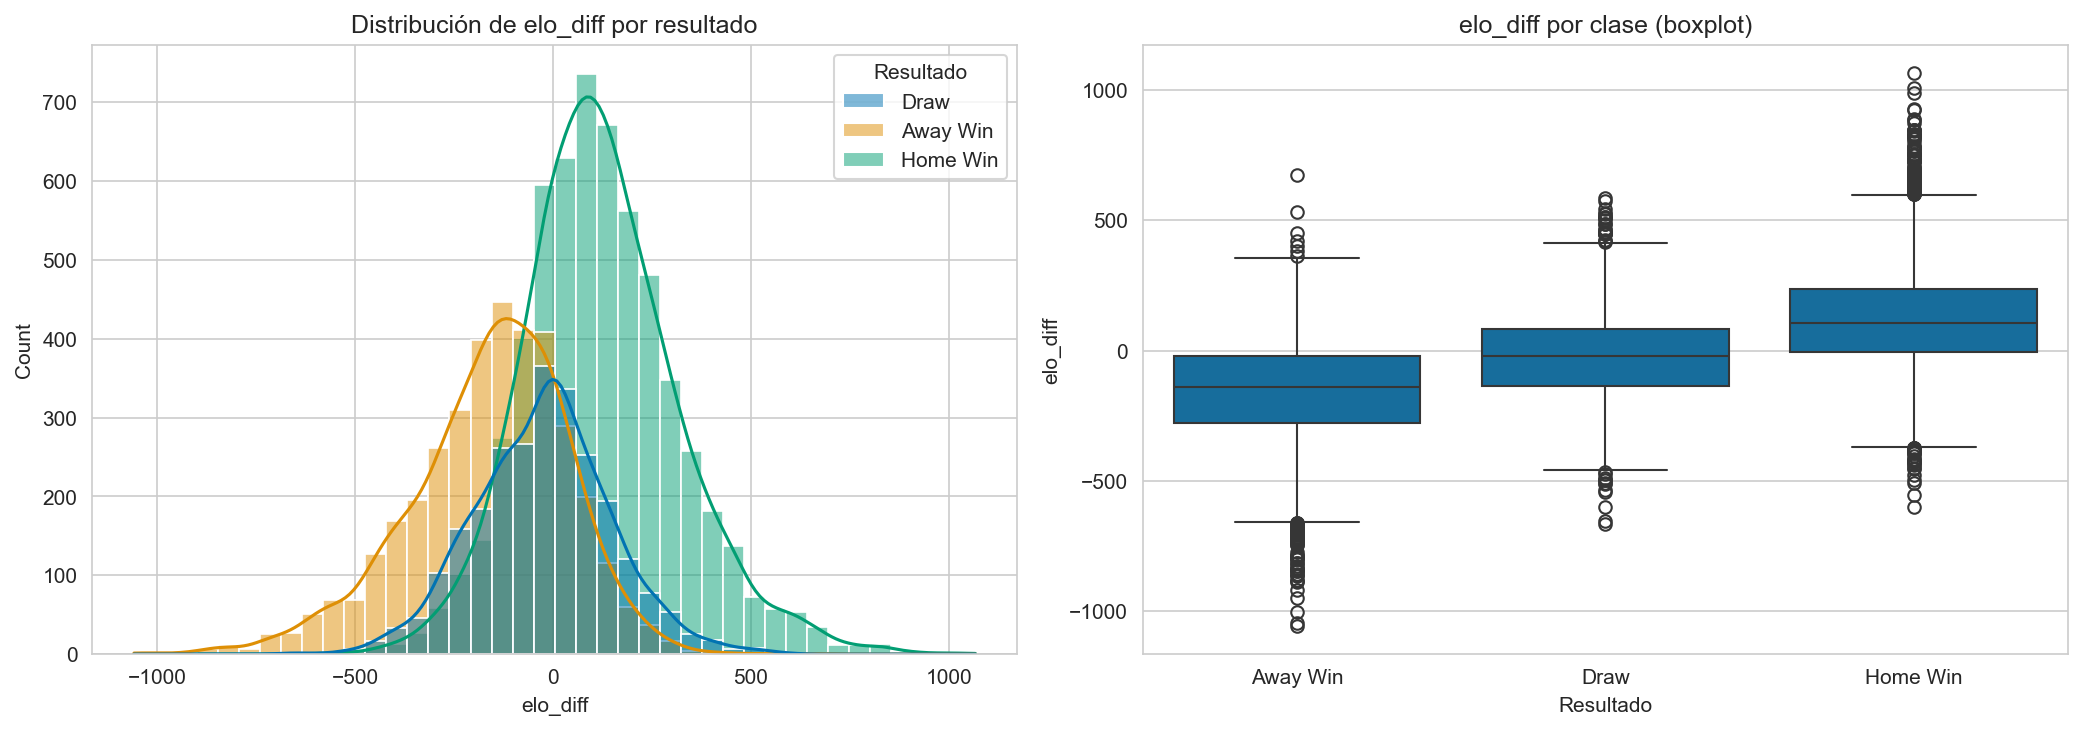
\includegraphics[width=\columnwidth]{eda_05_elo_diff.png}
  \caption{Distribuci\'on de \texttt{elo\_diff} por clase de resultado
    (H/E/V). La separaci\'on monot\'onica entre las tres distribuciones
    respalda el poder predictivo del feature.}
  \label{fig:elo_diff}
\end{figure}

\begin{figure}[!t]
  \centering
  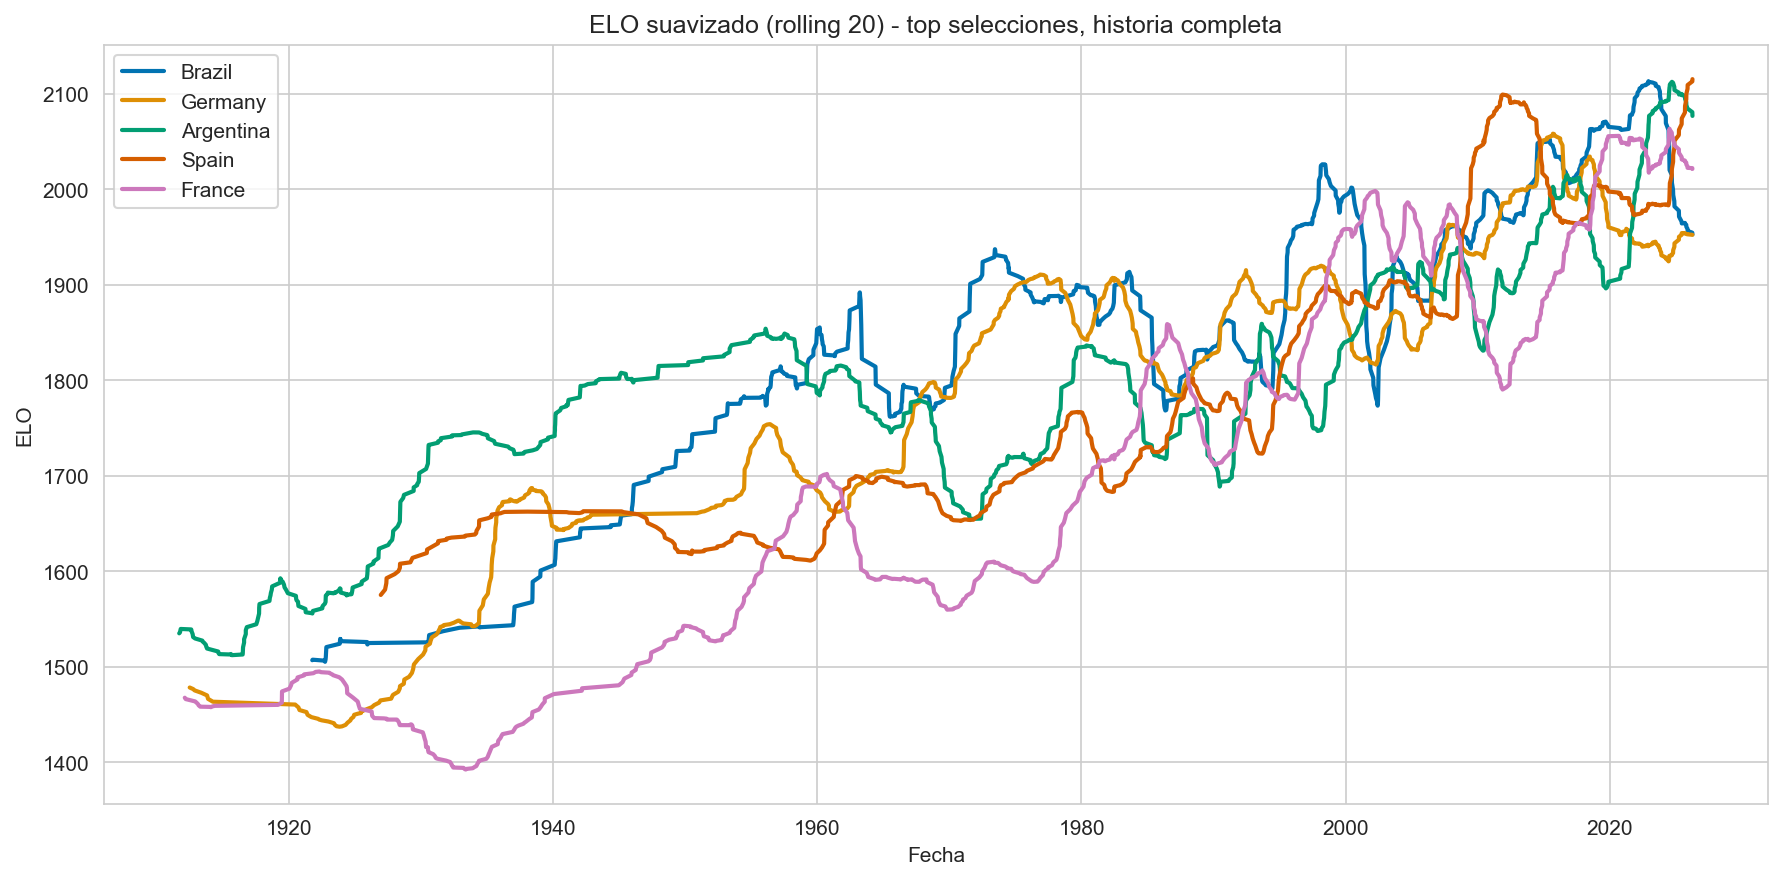
\includegraphics[width=\columnwidth]{eda_07_elo_history.png}
  \caption{Evoluci\'on del rating ELO para cinco selecciones
    representativas a lo largo de cuatro d\'ecadas.}
  \label{fig:elo_history}
\end{figure}

\subsection{Decaimiento temporal (sin rebalanceo de clases)}
\label{sec:timedecay}

Cada partido contribuye al entrenamiento con un peso
\begin{equation}
  W(t) \;=\; e^{-\lambda \,\Delta t},
  \quad \lambda = 1\times 10^{-3}\ \text{d\'ias}^{-1},
\end{equation}
donde $\Delta t$ son los d\'ias entre la fecha del partido y el horizonte
de referencia. Los pesos se renormalizan por su media para que el
aprendizaje permanezca a escala unitaria.

\textbf{Por qu\'e NO se rebalancean las clases.} La v1 multiplicaba
adem\'as por el peso \texttt{balanced} de \texttt{sklearn} para
``corregir'' el desbalance natural $H\!\approx\!47$\,\%,
$E\!\approx\!21$\,\%, $V\!\approx\!32$\,\% (Fig.\ \ref{fig:target}).
Rebalancear clases es una t\'ecnica para clasificaci\'on dura con clases
raras; cuando el objetivo son \emph{probabilidades calibradas} evaluadas
con log-loss, deforma las posteriores alej\'andolas de las tasas base
(los empates se sobreponderaban ${\sim}1{,}6\times$, produciendo una
sobrepredicci\'on media de $+3{,}5$ puntos porcentuales en la clase
empate). Eliminar el rebalanceo mejora el log-loss de test de todos los
modelos; para el XGBoost con hiperpar\'ametros fijos la mejora es de
${,}8547$ a ${,}8443$ y la sobrepredicci\'on de empates desaparece. El
desbalance de clases NO se ``corrige'' porque no es un defecto: es la
distribuci\'on real del fen\'omeno que el modelo debe estimar.

\begin{figure}[!t]
  \centering
  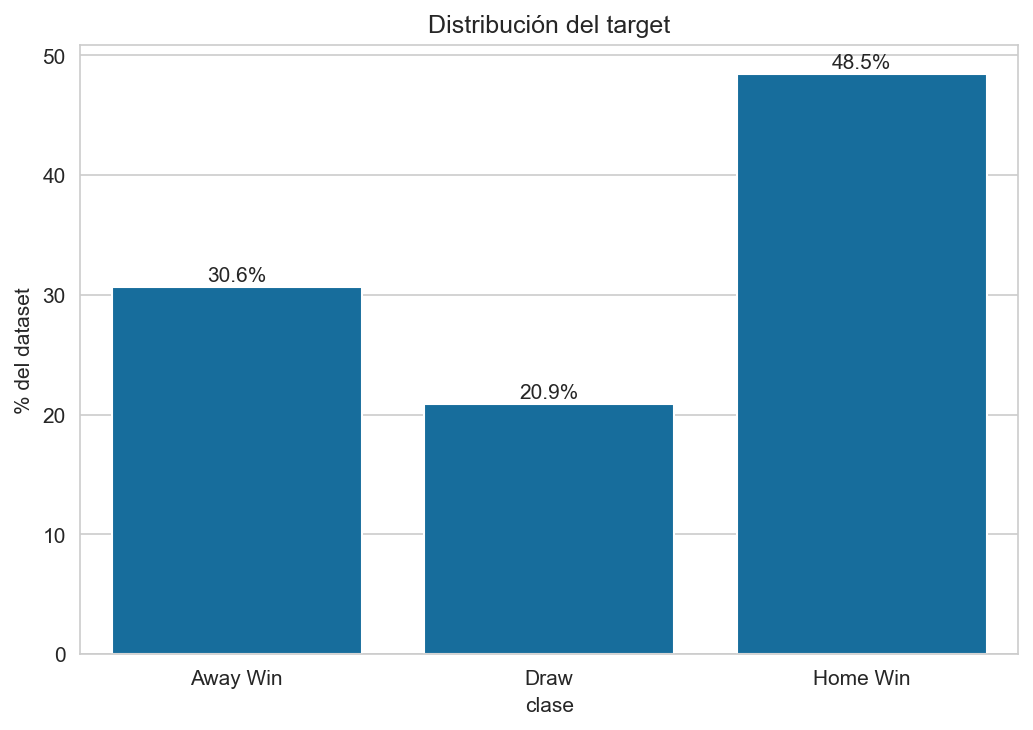
\includegraphics[width=\columnwidth]{eda_04_target_distribution.png}
  \caption{Distribuci\'on de la variable objetivo. El desbalance hacia la
    clase \emph{Local} motiva la ponderaci\'on \texttt{class\_weight=\,balanced}.}
  \label{fig:target}
\end{figure}

\begin{figure*}[!t]
  \centering
  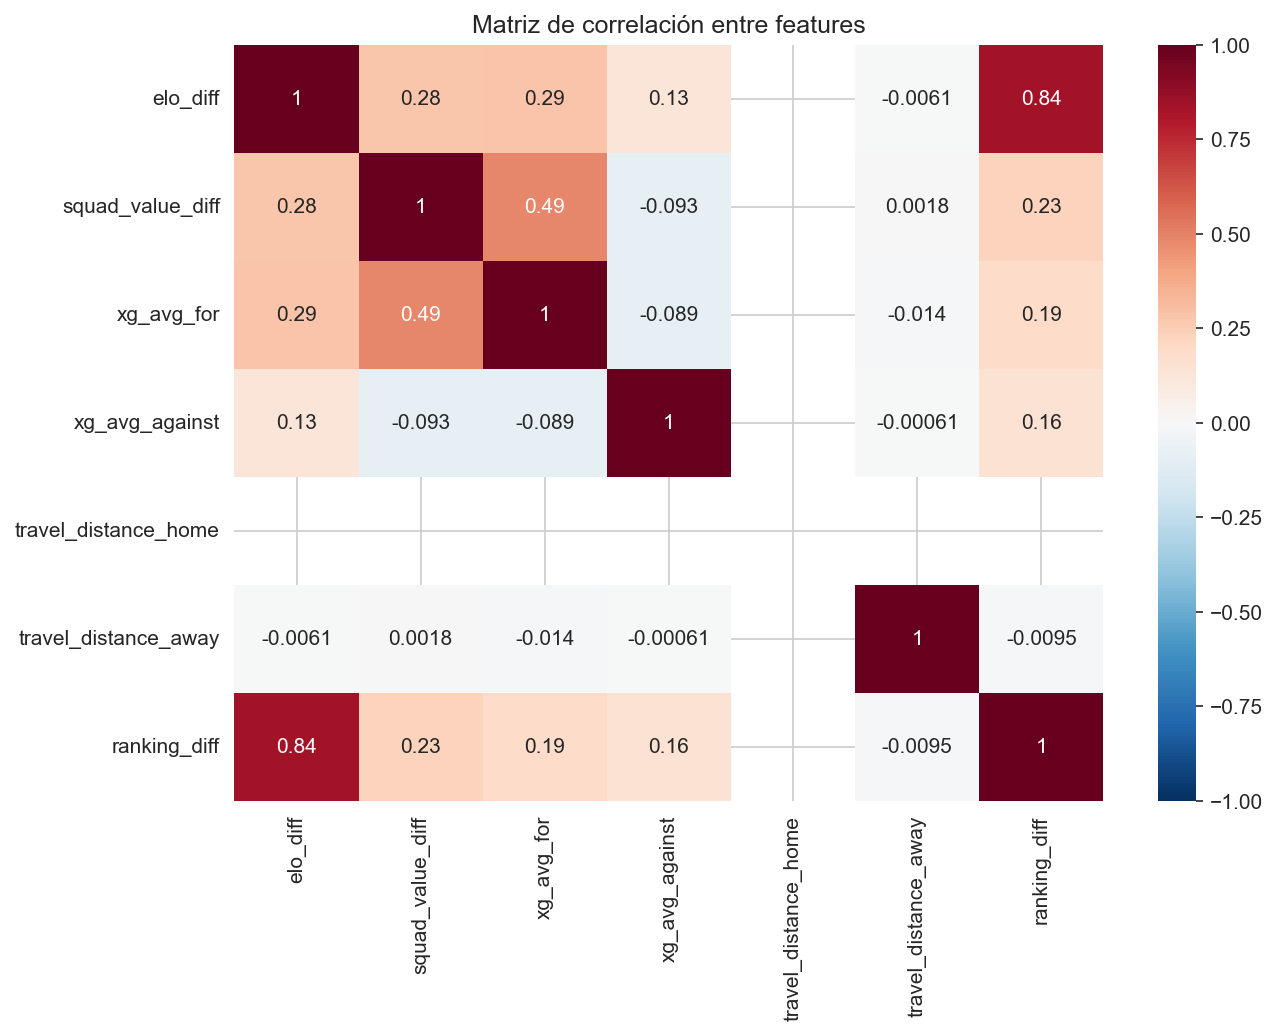
\includegraphics[width=0.65\textwidth]{eda_06_correlation_matrix.png}
  \caption{Matriz de correlaci\'on de las caracter\'isticas evaluadas
    (incluye, por completitud, las retiradas en v2). Se observa
    colinealidad alta entre \texttt{elo\_diff} y \texttt{ranking\_diff} ($r=0{,}88$)
    y una anti-correlaci\'on de \texttt{striker\_concentration\_diff} con la fuerza
    ($\approx-0{,}37$): los equipos fuertes reparten m\'as el goleo.}
  \label{fig:corr}
\end{figure*}

\section{Modelado}
\label{sec:modeling}

El problema se formula como clasificaci\'on multiclase a nivel de
partido $\{H,E,V\}$. Se entrenan tres familias: Regresi\'on Log\'istica
multinomial (con \texttt{StandardScaler}), XGBoost
(\texttt{multi:softprob}) y LightGBM. La b\'usqueda de hiperpar\'ametros
emplea Optuna \cite{akiba2019optuna} con $100$ \emph{trials} y
\texttt{TimeSeriesSplit}$(n=5)$ interno sobre el conjunto de
entrenamiento, optimizando \texttt{neg\_log\_loss}. La Fig.\
\ref{fig:shap} resume la importancia SHAP agregada (mean |SHAP|) del
XGBoost y muestra que \texttt{elo\_diff} domina la contribuci\'on por un
orden de magnitud. La cautela interpretativa es obligada:
\texttt{elo\_diff} y \texttt{ranking\_diff} son altamente colineales
($r\approx 0{,}88$) y SHAP reparte cr\'edito de forma inestable entre
features correlacionadas, de modo que el orden de las features menores no
soporta conclusiones; la cuantificaci\'on rigurosa de aportes se delega al
estudio de ablaci\'on multi-semilla (\S\ref{sec:ablation}).

\begin{figure}[!t]
  \centering
  
\includegraphics[width=\columnwidth]{shap_summary.png}
  \caption{Resumen SHAP agregado (mean |SHAP|) del XGBoost. \texttt{elo\_diff}
    domina la contribuci\'on, con \texttt{striker\_concentration\_diff} en segundo
    lugar y \texttt{ranking\_diff} en tercero.}
  \label{fig:shap}
\end{figure}

\subsection{Divisi\'on temporal y selecci\'on del modelo}

El split es estrictamente temporal (Tabla \ref{tab:split}). La franja de
validaci\'on 2021 se subdivide a su vez 70/30: el primer 70\,\%
(val-cal) ajusta la calibraci\'on Platt del XGBoost y el 30\,\% final
(val-sel) decide el modelo final por log-loss. Esta subdivisi\'on evita
un sesgo sutil: comparar el modelo calibrado sobre los mismos datos donde
se ajust\'o su sigmoide lo favorecer\'ia espuriamente. El conjunto de
prueba no interviene en ninguna decisi\'on. En la corrida reportada,
val-sel selecciona la \textbf{regresi\'on log\'istica multinomial} como
modelo final --- un resultado coherente con la ablaci\'on
(\S\ref{sec:ablation}): la se\~nal \'util es esencialmente lineal en
\texttt{elo\_diff}.

\begin{table}[!t]
  \caption{Split temporal y uso de cada conjunto}
  \label{tab:split}
  \centering
  \renewcommand{\arraystretch}{1.15}
  \footnotesize
  \begin{tabular}{@{}L{1.7cm}L{2.6cm}L{3.1cm}@{}}
    \toprule
    \textbf{Conjunto} & \textbf{Filtro}                               & \textbf{Uso}                  \\
    \midrule
    Train             & \texttt{date < 2021-01-01}                    & LogReg, XGBoost, LightGBM     \\
    Val-cal           & primer 70\,\% de 2021                         & Calibraci\'on Platt (sigmoid) \\
    Val-sel           & \'ultimo 30\,\% de 2021                       & Selecci\'on del modelo final  \\
    Test              & \texttt{date $\ge$ 2022-01-01}                & Evaluaci\'on final            \\
    \bottomrule
  \end{tabular}
\end{table}

\textbf{Recorte m\'inimo.} El entrenamiento usa partidos con
\texttt{date $\geq$ 2010}, aunque \texttt{features.csv} contiene datos
desde 1993. Los features est\'aticos (xG, valor de plantilla, ranking
moderno) no son representativos del f\'utbol pre-2010, y el time decay
con $\lambda\!=\!{,}001$ ya reduce el peso de esos partidos a menos del
2\,\%. El ELO sigue calcul\'andose sobre el hist\'orico completo para
mayor precisi\'on.

\textbf{Doble pipeline.} Para validar el Mundial 2022 sin leakage se
re-ejecuta el entrenamiento con \texttt{cutoff = 2022-01-01} y, de forma
crucial, \textbf{sin las features anacr\'onicas} (xG y valor de
plantilla, que son \emph{snapshots} de ${\sim}2026$): un modelo
``pre-2022'' cuyo vector de entrada contiene informaci\'on observada en
2026 no constituye una validaci\'on out-of-time honesta aunque el target
sea limpio. El pipeline limpio usa solo \texttt{elo\_diff},
\texttt{ranking\_diff} y las dos features de eventos as-of-date.

\section{Motor de simulaci\'on del torneo}
\label{sec:simulation}

El motor (\texttt{src/simulation/}) ejecuta $N{=}10{,}000$ realizaciones
del torneo completo. El bracket eliminatorio se carga como \emph{dato}
(\texttt{wc2026\_bracket.csv}), transcrito del calendario oficial FIFA
\cite{fifa2026,wiki_knockout}: de los 16 partidos del \emph{Round of 32},
8 enfrentan ganadores de grupo contra los mejores terceros (cada partido
con un \emph{pool} oficial de grupos de procedencia), 4 enfrentan
ganadores contra segundos y 4 cruzan segundos entre s\'i. La versi\'on v1
de este trabajo usaba un bracket inventado con cuatro cruces
tercero-vs-tercero --- inexistentes en el reglamento --- que garantizaba
exactamente 4 terceros en octavos y endurec\'ia el camino de los
favoritos; su correcci\'on cambia materialmente la progresi\'on. Cada
partido pasa por las siguientes etapas:

\begin{enumerate}
  \item \textbf{Probabilidades sim\'etricas con localía por sede.} Se
        promedia $P(i\text{ vs }j)$ con la inversi\'on de
        $P(j\text{ vs }i)$ para eliminar el sesgo home/away del dataset,
        salvo cuando un anfitri\'on juega \emph{en su propio pa\'is}
        seg\'un la sede del calendario (M\'exico en una sede de EE.UU.\
        no recibe localía; la v1 no verificaba la sede).
  \item \textbf{Marcador condicionado al outcome.} El \emph{outcome}
        $\{H,E,V\}$ se sortea con las probabilidades del modelo y el
        marcador se muestrea de la distribuci\'on conjunta Poisson
        independiente ($\mu$ basado en xG) \emph{condicionada} a ese
        outcome (truncada y renormalizada sobre la grilla $0$--$10$).
        Esto reemplaza la reconciliaci\'on ad-hoc de la v1
        ($g_i \leftarrow g_j{+}1$), que distorsionaba la distribuci\'on
        de DG/GF justo donde deciden los desempates.
  \item \textbf{Fase de grupos.} $12$ grupos de $4$; clasifican los dos
        primeros m\'as los $8$ mejores terceros. Desempates seg\'un
        reglamento: \textbf{puntos $\to$ DG $\to$ GF $\to$ enfrentamiento
        directo $\to$ sorteo} (con el RNG de la iteraci\'on; la v1 dejaba
        el orden de inserci\'on, un sesgo determinista). El \emph{fair
        play} no es simulable y se omite (aproximaci\'on documentada).
  \item \textbf{Asignaci\'on de terceros.} Los 8 mejores terceros se
        asignan a los 8 slots del R32 mediante un \emph{matching} exacto
        que respeta los pools oficiales de procedencia (la tabla FIFA de
        495 combinaciones es una elecci\'on particular entre los
        matchings v\'alidos; no est\'a publicada en forma compacta).
  \item \textbf{Eliminatorias.} \emph{Round of 32} $\to$ \emph{Round of
        16} $\to$ Cuartos $\to$ Semifinales $\to$ Final, con la
        progresi\'on de llaves y sedes del calendario oficial. Si hay
        empate tras los $90'$, la definici\'on por penales se modela como
        $\text{Bernoulli}(0{,}5)$.
\end{enumerate}

Se contabilizan, por equipo, las veces que alcanza cada ronda y los
intervalos de confianza al 95\,\% se calculan con el m\'etodo binomial
exacto de Clopper--Pearson \cite{clopper1934} v\'ia
\texttt{scipy.stats.beta}. Las $N$ iteraciones, independientes entre s\'i, se
reparten en bloques fijos ejecutados en paralelo (\texttt{joblib}); cada bloque
usa un \emph{stream} RNG propio derivado de
\texttt{SeedSequence(seed).spawn}, de modo que el resultado es \textbf{id\'entico
  con cualquier n\'umero de \emph{workers}} (reproducibilidad independiente del
paralelismo).

\section{Evaluaci\'on}
\label{sec:eval}

Se reportan Log-Loss y Brier score sobre el conjunto de prueba
($\texttt{date}\ge 2022$). Se evita \texttt{accuracy} por ser
inadecuada para predicciones probabil\'isticas desbalanceadas
\cite{brier1950}.

\textbf{Nota metodol\'ogica sobre el Brier.} El valor reportado es el
promedio de los tres scores binarios \emph{one-vs-rest} (cada clase
$\{H,E,V\}$ contra el resto), de modo que se sit\'ua en el rango
$[0,1]$ y no en la formulaci\'on multiclase de suma de diferencias
cuadr\'aticas (rango $[0,2]$). Ambas medidas son equivalentes salvo un
factor: el Brier de suma multiclase es $K$ veces el promediado, con
$K=3$ clases; as\'i, el ${,}163$ reportado corresponde a ${,}490$ en
la escala $[0,2]$.

La Tabla \ref{tab:eval} reporta las m\'etricas puntuales junto con el
delta de log-loss frente al mejor modelo y su IC al $95\,\%$ por
\emph{bootstrap} pareado por partido ($2{,}000$ r\'eplicas): los puntos
sin intervalo no permiten afirmar que un modelo ``gana''. LightGBM y la
regresi\'on log\'istica quedan \textbf{estad\'isticamente empatados} en
primer lugar; ambos superan significativamente al XGBoost. Como
referencia, el baseline de priors de clase da $1{,}050$ y el uniforme
$\ln(3) = 1{,}099$; el mejor modelo de la v1 (con rebalanceo) daba
${,}8547$.

\textbf{La calibraci\'on Platt deja de ser necesaria.} En la v1, la
calibraci\'on ``correg\'ia la sobreconfianza'' del XGBoost
(${,}866\!\to\!{,}855$). El diagn\'ostico era incorrecto: lo que la
sigmoide reparaba parcialmente era la deformaci\'on introducida por el
propio rebalanceo de clases. Entrenando sobre la distribuci\'on natural,
el XGBoost calibrado es \emph{peor} que el crudo (${,}8716$ vs
${,}8587$): con un a\~no de validaci\'on, la sigmoide a\~nade varianza
sin sesgo que corregir. La selecci\'on en val-sel resuelve esta decisi\'on
sin juicio manual.

\begin{table}[!t]
  \caption{Evaluaci\'on sobre test temporal ($\ge$2022, $n{=}2{,}208$).
    $\Delta$LL vs mejor con IC95 bootstrap pareado.}
  \label{tab:eval}
  \centering
  \renewcommand{\arraystretch}{1.15}
  \small
  \begin{tabular}{@{}lccc@{}}
    \toprule
    \textbf{Modelo} & \textbf{Log-Loss} $\downarrow$ & \textbf{Brier} $\downarrow$ & \textbf{$\Delta$LL [IC95]} \\
    \midrule
    \textbf{LightGBM} & \textbf{{,}8356} & \textbf{{,}1634} & ---                            \\
    \textbf{LogReg}   & \textbf{{,}8360} & {,}1635          & $+{,}000\,[-{,}007,+{,}009]$   \\
    XGBoost           & {,}8587          & {,}1678          & $+{,}023\,[+{,}015,+{,}031]^*$ \\
    XGBoost-Cal       & {,}8716          & {,}1699          & $+{,}036\,[+{,}026,+{,}046]^*$ \\
    \bottomrule
  \end{tabular}

  \vspace{2pt}
  {\scriptsize $^*$ significativo (el IC95 excluye el cero).}
\end{table}

\begin{figure}[!t]
  \centering
  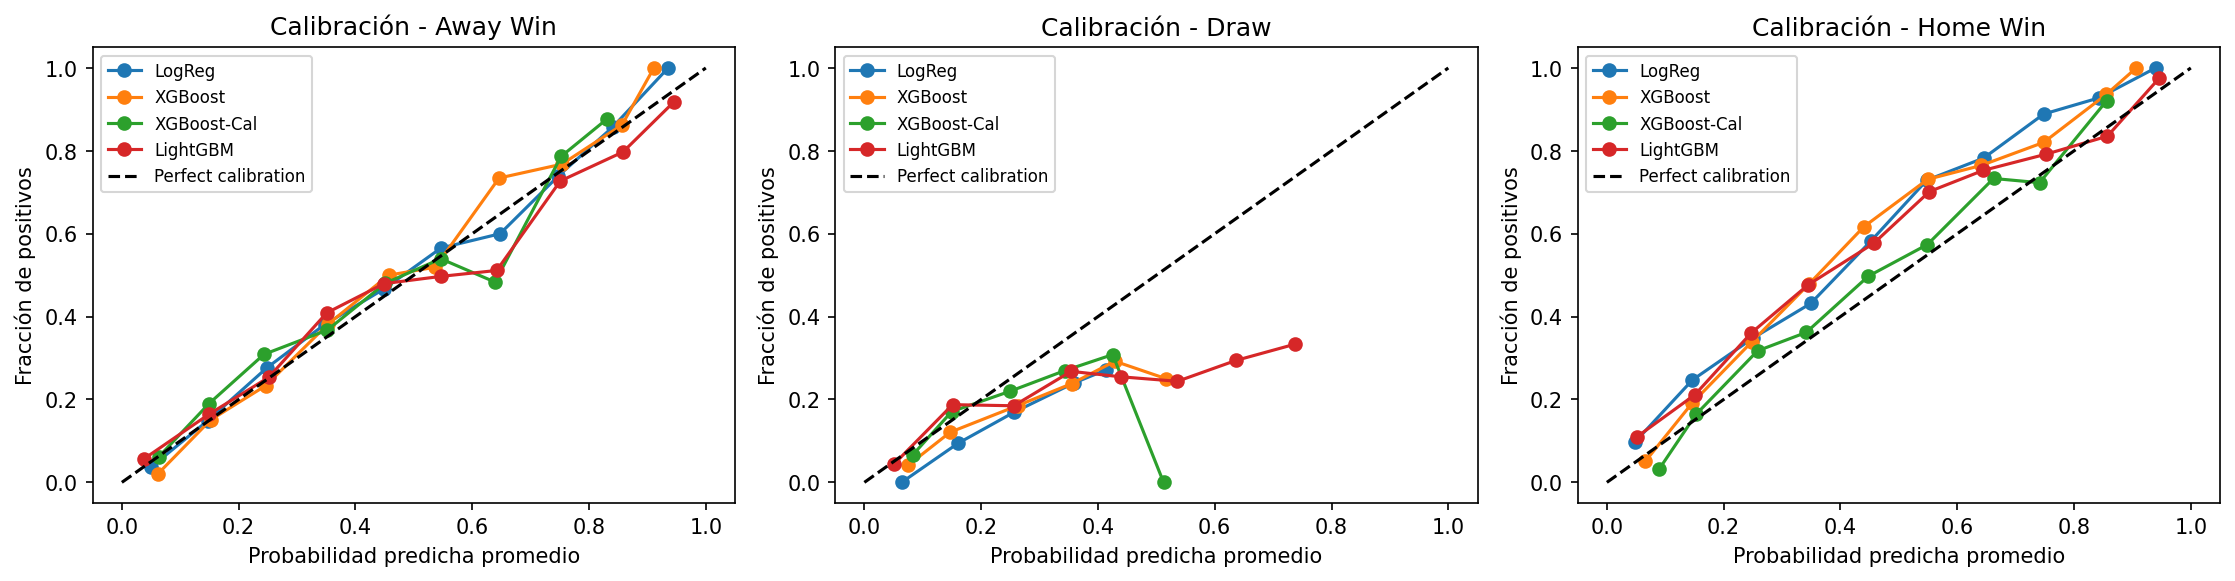
\includegraphics[width=\columnwidth]{calibration_curves.png}
  \caption{Curvas de calibraci\'on por clase. Todos los modelos se
    aproximan bien a la diagonal en \emph{Away Win} y \emph{Home Win};
    la clase \emph{Draw} queda sub-calibrada en todos — reflejo directo
    de la baja correlaci\'on entre features y empates ($|r|<0{,}07$).}
  \label{fig:calibration}
\end{figure}

\subsection{Estudio de ablaci\'on}
\label{sec:ablation}

Para cuantificar la contribuci\'on de cada grupo de features se
reentrena el XGBoost calibrado con \textbf{diez semillas por
configuraci\'on}, manteniendo fijos el split, los pesos y los
hiperpar\'ametros; se reporta media $\pm$ desviaci\'on del log-loss y un
\emph{bootstrap} pareado (por partido, sobre la p\'erdida promediada
entre semillas) del delta frente al modelo completo. La v1 reportaba
corridas \'unicas y conclu\'ia que las features est\'aticas y las
derivadas ``aportaban'' $+0{,}004$; con repeticiones y un IC, esa
conclusi\'on no sobrevive. La Tabla \ref{tab:ablation} muestra el
resultado, incisivo: \textbf{ning\'un grupo de features a\~nade se\~nal
significativa sobre el resto, y la configuraci\'on de una sola feature
(\texttt{elo\_diff}) es significativamente MEJOR que el modelo completo}
($\Delta\text{LL} = -0{,}011$, IC95 $[-0{,}020, -0{,}002]$). En esta
arquitectura y con este volumen de datos, las seis features adicionales
introducen m\'as varianza que se\~nal. Este hallazgo es coherente con la
selecci\'on del modelo final (una log\'istica, esencialmente lineal en
\texttt{elo\_diff}) y reencuadra el papel del resto del pipeline: las
features adicionales se conservan como instrumentaci\'on documentada,
no como fuentes demostradas de se\~nal.

\begin{table}[!t]
  \caption{Ablaci\'on multi-semilla (XGBoost calibrado, 10 seeds,
    test $\ge$2022). $\Delta$LL vs completo con IC95 bootstrap pareado.}
  \label{tab:ablation}
  \centering
  \renewcommand{\arraystretch}{1.15}
  \scriptsize
  \begin{tabular}{@{}L{2.5cm}ccc@{}}
    \toprule
    \textbf{Configuraci\'on}  & \textbf{LL (media$\pm$sd)} & \textbf{$\Delta$LL [IC95]} & \textbf{Signif.} \\
    \midrule
    Completo (7 feat.)         & ${,}8675\pm{,}0015$ & ---                              & ---         \\
    Sin xG                     & ${,}8667\pm{,}0017$ & $-{,}001\,[-{,}006,+{,}005]$     & no          \\
    Sin squad\_value           & ${,}8689\pm{,}0020$ & $+{,}002\,[-{,}001,+{,}004]$     & no          \\
    Sin derivadas              & ${,}8623\pm{,}0013$ & $-{,}005\,[-{,}011,+{,}001]$     & no          \\
    Sin penalty\_share         & ${,}8639\pm{,}0016$ & $-{,}004\,[-{,}007,+{,}000]$     & no          \\
    Sin est\'aticas (xG+squad) & ${,}8656\pm{,}0014$ & $-{,}002\,[-{,}007,+{,}004]$     & no          \\
    Solo \texttt{elo\_diff}    & ${,}8566\pm{,}0007$ & $-{,}011\,[-{,}020,-{,}002]$ & \textbf{s\'i} \\
    \bottomrule
  \end{tabular}
\end{table}

\textbf{Validaci\'on hist\'orica (sin leakage).} El pipeline
\texttt{\_pre2022} --- entrenado solo con \texttt{date<2022-01-01} y sin
las features anacr\'onicas --- se eval\'ua sobre los partidos de 2022
como prueba \emph{out-of-time} en la que ni el modelo ni el vector de
entrada ven informaci\'on posterior al cutoff: log-loss $0{,}985$,
accuracy $54{,}4\,\%$. La cifra es peor que la del test principal ---
exactamente lo esperable al retirar el leakage de los snapshots, y la
raz\'on de reportarla: el test principal, que s\'i recibe los snapshots
de 2026, debe leerse como \textbf{cota optimista}.

\section{Resultados de la simulaci\'on}
\label{sec:results}

La Tabla \ref{tab:top10} lista el Top-10 de candidatos al t\'itulo junto a
la probabilidad impl\'icita del mercado, y la Tabla \ref{tab:hosts} resume
la progresi\'on por fase de los tres anfitriones. \textbf{Semántica de los
intervalos:} el IC de Clopper--Pearson cuantifica \'unicamente el error
de muestreo Monte Carlo --- reducible corriendo m\'as iteraciones --- y
NO la incertidumbre del modelo. Para esta \'ultima, el modo
\texttt{--ensemble} reentrena $K$ r\'eplicas \emph{bootstrap} del modelo
final y reporta el rango de P(campe\'on) entre r\'eplicas
(\texttt{simulation\_ensemble.csv}), que es sustancialmente m\'as ancho.

\begin{table}[!t]
  \caption{Top-10 candidatos a campe\'on (10\,000 iteraciones, IC
    Clopper--Pearson de simulaci\'on) y mercado des-vigorizado}
  \label{tab:top10}
  \centering
  \renewcommand{\arraystretch}{1.15}
  \small
  \begin{tabular}{@{}lccc@{}}
    \toprule
    \textbf{Equipo} & \textbf{P(Campe\'on)} & \textbf{IC 95\,\% sim.} & \textbf{Mercado} \\
    \midrule
    Espa\~na        & 27{,}46\,\%           & [26{,}59, 28{,}35] & 14{,}9\,\% \\
    Argentina       & 13{,}78\,\%           & [13{,}11, 14{,}47] &  8{,}2\,\% \\
    Francia         & 11{,}65\,\%           & [11{,}03, 12{,}29] & 13{,}7\,\% \\
    Inglaterra      &  7{,}73\,\%           & [ 7{,}21,  8{,}27] & 10{,}2\,\% \\
    Alemania        &  3{,}61\,\%           & [ 3{,}25,  3{,}99] &  5{,}5\,\% \\
    Pa\'ises Bajos  &  3{,}05\,\%           & [ 2{,}72,  3{,}41] &  3{,}9\,\% \\
    Ecuador         &  3{,}05\,\%           & [ 2{,}72,  3{,}41] &  0{,}5\,\% \\
    Brasil          &  3{,}04\,\%           & [ 2{,}71,  3{,}40] &  9{,}1\,\% \\
    Colombia        &  3{,}00\,\%           & [ 2{,}67,  3{,}35] &  2{,}0\,\% \\
    Jap\'on         &  2{,}99\,\%           & [ 2{,}66,  3{,}34] &  1{,}6\,\% \\
    \bottomrule
  \end{tabular}
\end{table}

\begin{table}[!t]
  \caption{Progresi\'on por fase de los anfitriones (\%)}
  \label{tab:hosts}
  \centering
  \renewcommand{\arraystretch}{1.15}
  \begin{tabular}{@{}lccc@{}}
    \toprule
    \textbf{Fase} & \textbf{M\'exico} & \textbf{EE.UU.} & \textbf{Canad\'a} \\
    \midrule
    Round of 32   & 96{,}3            & 74{,}7          & 97{,}2            \\
    Round of 16   & 61{,}5            & 44{,}5          & 61{,}9            \\
    Cuartos       & 28{,}4            & 21{,}0          & 30{,}1            \\
    Semifinales   & 11{,}3            & 7{,}8           & 10{,}1            \\
    Final         & 4{,}0             & 3{,}0           & 3{,}8             \\
    Campe\'on     & 1{,}2             & 1{,}0           & 1{,}2             \\
    \bottomrule
  \end{tabular}
\end{table}

\subsection{Benchmark contra el mercado de apuestas}
\label{sec:benchmark}

Siguiendo la pr\'actica est\'andar de la literatura
\cite{dixon1997}, las probabilidades del modelo se contrastan con las
impl\'icitas del mercado (BetMGM, snapshot 2026-06-10, des-vigorizado por
normalizaci\'on proporcional; \emph{overround} $1{,}22$). La distancia de
variaci\'on total entre ambas distribuciones es $0{,}27$. El patr\'on de
divergencia es sistem\'atico: el modelo \textbf{sobrepondera al l\'ider
de ELO} (Espa\~na $27{,}5$\,\% vs $14{,}9$\,\%; Argentina $13{,}8$\,\% vs
$8{,}2$\,\%) e \textbf{infrapondera a equipos cuya calidad percibida
excede su ELO reciente} (Brasil $3{,}0$\,\% vs $9{,}1$\,\%; Portugal
$2{,}7$\,\% vs $8{,}2$\,\%). La causa es estructural: la se\~nal del
modelo es esencialmente \texttt{elo\_diff} amplificada sobre siete rondas
de torneo, sin \emph{shrinkage} hacia el consenso ni informaci\'on de
plantillas que el mercado s\'i incorpora. Se reporta como limitaci\'on
abierta en lugar de ajustar el modelo hacia el mercado ex-post.

\subsection{An\'alisis de sensibilidad a lesiones}

Las lesiones no se modelan estructuralmente;
\texttt{src/analysis/sensitivity.py} aplica un escenario de crisis
agregado al top-5 y re-ejecuta la simulaci\'on. La v1 perturbaba
\'unicamente \texttt{squad\_value} ($-30$\,\%) --- la feature de
\emph{menor} importancia del modelo --- por lo que su resultado
($|\Delta|\!\leq\!0{,}4$ pp) estaba predeterminado por el dise\~no. El
escenario v2 perturba conjuntamente los tres canales por los que una
crisis de lesiones se manifiesta en el espacio de features:
\texttt{squad\_value} $-30$\,\%, \texttt{xg\_for} $-10$\,\% y ELO $-25$
puntos. La Tabla \ref{tab:sens} muestra efectos ahora materiales y
monot\'onicos con la probabilidad base.

\begin{table}[!t]
  \caption{Sensibilidad al escenario conjunto de lesiones
    (squad $-30$\,\%, xG $-10$\,\%, ELO $-25$)}
  \label{tab:sens}
  \centering
  \renewcommand{\arraystretch}{1.15}
  \begin{tabular}{@{}lccc@{}}
    \toprule
    \textbf{Equipo} & \textbf{Base \%} & \textbf{Lesi\'on \%} & \textbf{$\Delta$ pp} \\
    \midrule
    Espa\~na        & 27{,}46          & 22{,}19              & $-5{,}27$            \\
    Argentina       & 13{,}78          & 9{,}52               & $-4{,}26$            \\
    Francia         & 11{,}65          & 9{,}26               & $-2{,}39$            \\
    Inglaterra      & 7{,}73           & 6{,}01               & $-1{,}72$            \\
    Alemania        & 3{,}61           & 2{,}46               & $-1{,}15$            \\
    \bottomrule
  \end{tabular}
\end{table}

\subsection{Incertidumbre del modelo (ensemble bootstrap)}

Reentrenando $K{=}5$ r\'eplicas \emph{bootstrap} del modelo final y
simulando $2{,}000$ iteraciones con cada una, el rango de P(campe\'on)
entre r\'eplicas resulta mucho m\'as ancho que el IC de simulaci\'on:
para Espa\~na, $[23{,}6, 29{,}9]$ entre modelos frente a
$[26{,}1, 27{,}8]$ de Clopper--Pearson. La incertidumbre dominante del
pron\'ostico es la del modelo, no la del Monte Carlo --- raz\'on por la
que reportar \'unicamente intervalos de simulaci\'on (como la v1)
transmite una precisi\'on espuria.

\section{Limitaciones}
\label{sec:limits}

El modelo presenta seis limitaciones reconocidas:

\begin{enumerate}
  \item \textbf{Debutantes.} Equipos como Uzbekist\'an, Curazao o Cabo
        Verde tienen historial internacional escaso; su ELO se inicializa con
        el valor neutro $1500$ y converge lentamente, lo que probablemente
        \emph{infla} su probabilidad relativa frente a rivales subestimados de
        la misma confederaci\'on.
  \item \textbf{Cobertura xG.} El \emph{open data} de StatsBomb
        \cite{statsbomb} privilegia torneos UEFA/CONMEBOL; 13 de las 48
        selecciones reciben el xG por defecto de $1{,}2$ (media global), lo
        que subestima la varianza inter-equipos fuera de Europa.
  \item \textbf{Features est\'aticas anacr\'onicas en el pipeline
        principal.} El xG y el valor de plantilla son \emph{snapshots} de
        ${\sim}2026$ aplicados a todos los partidos, \emph{incluido el
        test}: las m\'etricas del test principal son por tanto una cota
        optimista. La cifra de referencia limpia es la validaci\'on WC2022
        del pipeline \texttt{\_pre2022}, que las excluye. A diferencia de
        lo afirmado en la v1, S\'I existe serie hist\'orica de valores de
        Transfermarkt; versionarla es trabajo futuro.
  \item \textbf{Concentraci\'on de se\~nal y divergencia con el
        mercado.} La se\~nal \'util es esencialmente \texttt{elo\_diff}
        (la ablaci\'on multi-semilla no encuentra aporte significativo de
        ning\'un otro grupo), y su amplificaci\'on sobre siete rondas
        produce favoritos m\'as extremos que el mercado de apuestas
        (\S\ref{sec:benchmark}), sin \emph{shrinkage} hacia el consenso.
  \item \textbf{Asignaci\'on de terceros aproximada.} El matching de
        terceros respeta los pools oficiales por partido, pero la tabla
        FIFA exacta de 495 combinaciones no est\'a publicada en forma
        compacta; entre matchings v\'alidos se elige el primero en orden
        determinista. El \emph{fair play} tampoco se simula como criterio
        de desempate.
  \item \textbf{Lesiones de \'ultima hora.} No hay modelado estructural
        de bajas individuales; \texttt{sensitivity.py} es un \emph{stress
        test} agregado (squad $-30$\,\%, xG $-10$\,\%, ELO $-25$). Una baja
        clave en una posici\'on espec\'ifica (e.g., portero titular) tiene
        un impacto que el modelo no puede capturar.
\end{enumerate}

\section{Reproducibilidad}
\label{sec:reproducibility}

El repositorio mantiene una arquitectura modular bajo \texttt{src/}
(\texttt{data/}, \texttt{features/}, \texttt{models/}, \texttt{simulation/},
\texttt{analysis/}, \texttt{visualization/}). Los CSVs versionables
se producen en \texttt{data/processed/} y las figuras
en \texttt{reports/figures/}. Toda la cadena se reproduce con:

\begin{verbatim}
pip install -e .
make all   # features -> train -> evaluate
           # -> simulate -> sensitivity
python -m src.analysis.ablation --seeds 10
python -m src.simulation.simulate \
  --iterations 10000 --ensemble 5
python -m src.analysis.benchmark
streamlit run \
  src/visualization/dashboard.py
\end{verbatim}

La cobertura de pruebas (\texttt{pytest tests/ -v}, 57 tests) valida la
mec\'anica del ELO (margen de victoria, ventaja de local condicionada a
sede neutral), la estructura oficial del bracket (sin cruces
tercero-vs-tercero, pools respetados), el matching de terceros sobre
combinaciones muestreadas, la coherencia del Poisson condicionado con el
outcome sorteado, los desempates por sorteo v\'ia RNG y el c\'alculo
as-of-date de las features de eventos. Los resultados de la v1 quedan
congelados en \texttt{data/processed/baseline\_v1/} y cualquier cambio se
acepta solo con un delta de log-loss significativo seg\'un
\texttt{src/analysis/compare\_runs.py} (bootstrap pareado).

\section{Conclusiones y trabajo futuro}
\label{sec:conclusion}

Se ha presentado un sistema reproducible para predecir la Copa Mundial
2026: m\'ultiples fuentes limpias, siete caracter\'isticas --dos de
eventos, calculadas \emph{as-of-date}--, \emph{benchmark} de cuatro
modelos con selecci\'on en validaci\'on y significancia por bootstrap
pareado, un motor Monte Carlo de $10{,}000$ iteraciones sobre el bracket
oficial, validaci\'on out-of-time sin leakage y contraste con el mercado.
El modelo final --- una regresi\'on log\'istica multinomial --- logra
Log-Loss de ${,}836$ en test, estad\'isticamente empatada con LightGBM y
significativamente mejor que el sistema v1 (${,}855$;
$\Delta = -0{,}019$, IC95 $[-0{,}030, -0{,}009]$).

El hallazgo metodol\'ogico central de esta revisi\'on es deflacionario y,
creemos, m\'as valioso que un ranking de features: con repeticiones e
intervalos, \textbf{ninguna feature m\'as all\'a de \texttt{elo\_diff}
aporta se\~nal demostrable} en este volumen de datos, y dos pr\'acticas
habituales --- el rebalanceo de clases y la calibraci\'on aplicada sin
diagn\'ostico del sesgo subyacente --- degradaban activamente las
probabilidades. Las simulaciones ubican a Espa\~na (27{,}5\,\%),
Argentina (13{,}8\,\%) y Francia (11{,}7\,\%) como favoritas, con la
advertencia expl\'icita de que el modelo es m\'as extremo que el mercado
en sus favoritos y de que la incertidumbre dominante es la del modelo
(rango ensemble de Espa\~na: $[23{,}6, 29{,}9]$), no la del Monte Carlo.

Trabajo futuro: (i) incorporar un modelo Dixon--Coles \cite{dixon1997}
para los marcadores en lugar de Poisson independiente condicionado;
(ii) versionar por temporada el valor de plantilla (la serie hist\'orica
de Transfermarkt existe) y reconstruir el test principal sin anacronismo;
(iii) \emph{shrinkage} de las probabilidades hacia el consenso del
mercado como modelo h\'ibrido, evaluado fuera de muestra; y (iv) modelar
lesiones a nivel de jugador integrando \emph{features} de minutos
disputados y posici\'on.

\section*{Disponibilidad de código y recursos}

El código fuente, los scripts de entrenamiento, los datos procesados y los
experimentos necesarios para reproducir los resultados de este estudio se
encuentran disponibles públicamente en \cite{repo}. Asimismo, se proporciona un
dashboard interactivo para la exploración de resultados y simulaciones
mediante \cite{dashboard}.

\hbadness=2800
\begin{thebibliography}{99}

  \bibitem{fifa2026}
  {F\'ed\'eration Internationale de Football Association}, ``{FIFA} World Cup
  2026 competition format and regulations,'' 2023. [Online]. Available:
  \url{https://www.fifa.com/fifaplus/en/tournaments/mens/worldcup/canadamexicousa2026}
  (accessed 2026-05-31).

  \bibitem{wiki_knockout}
  Wikipedia, ``2026 {FIFA} World Cup knockout stage,'' 2026. [Online].
  Available:
  \url{https://en.wikipedia.org/wiki/2026_FIFA_World_Cup_knockout_stage}
  (accessed 2026-06-10). Calendario oficial de partidos 73--104 con sedes y
  pools de terceros, transcrito en \texttt{data/raw/wc2026\_bracket.csv}.

  \bibitem{maher1982}
  M.~J. Maher, ``Modelling association football scores,'' \emph{Statistica
    Neerlandica}, vol.~36, no.~3, pp. 109--118, 1982, doi:
  \url{https://doi.org/10.1111/j.1467-9574.1982.tb00782.x}.

  \bibitem{dixon1997}
  M.~J. Dixon and S.~G. Coles, ``Modelling association football scores and
  inefficiencies in the football betting market,'' \emph{Journal of the Royal
    Statistical Society: Series C (Applied Statistics)}, vol.~46, no.~2, pp.
  265--280, 1997, doi: \url{https://doi.org/10.1111/1467-9876.00065}.

  \bibitem{elo1978}
  A.~E. Elo, \emph{The Rating of Chessplayers, Past and Present}.\hskip 1em plus
  0.5em minus 0.4em\relax New York: Arco Publishing, 1978.

  \bibitem{groll2019}
  A.~Groll, C.~Ley, G.~Schauberger, and H.~Van Eetvelde, ``A hybrid random
  forest to predict soccer matches in international tournaments,'' \emph{J.
    Quant. Anal. Sports}, vol.~15, no.~4, pp. 271--287, 2019, doi:
  \url{https://doi.org/10.1515/jqas-2018-0060}.

  \bibitem{chen2016xgboost}
  T.~Chen and C.~Guestrin, ``{XGBoost}: A scalable tree boosting system,'' in
  \emph{Proc. 22nd ACM SIGKDD Int. Conf. on Knowledge Discovery and Data
    Mining}, 2016, pp. 785--794, doi:
  \url{https://doi.org/10.1145/2939672.2939785}.

  \bibitem{ke2017lightgbm}
  G.~Ke \emph{et~al.}, ``{LightGBM}: A highly efficient gradient boosting
  decision tree,'' in \emph{Adv. Neural Inf. Process. Syst. (NeurIPS)},
  vol.~30, 2017.

  \bibitem{lundberg2017shap}
  S.~M. Lundberg and S.-I. Lee, ``A unified approach to interpreting model
  predictions,'' in \emph{Adv. Neural Inf. Process. Syst. (NeurIPS)}, vol.~30,
  2017.

  \bibitem{brier1950}
  G.~W. Brier, ``Verification of forecasts expressed in terms of probability,''
  \emph{Monthly Weather Review}, vol.~78, no.~1, pp. 1--3, 1950, doi:
  \url{https://doi.org/10.1175/1520-0493(1950)078<0001:VOFEIT>2.0.CO;2}.

  \bibitem{platt1999}
  J.~C. Platt, ``Probabilistic outputs for support vector machines and
  comparisons to regularized likelihood methods,'' in \emph{Advances in Large
    Margin Classifiers}, 1999, pp. 61--74.

  \bibitem{niculescu2005}
  A.~Niculescu-Mizil and R.~Caruana, ``Predicting good probabilities with
  supervised learning,'' in \emph{Proc. 22nd Int. Conf. on Machine Learning
    (ICML)}, 2005, pp. 625--632, doi:
  \url{https://doi.org/10.1145/1102351.1102430}.

  \bibitem{martj42}
  M.~J\"urisoo, ``International football results from 1872 to 2026
  (\texttt{results}, \texttt{goalscorers}, \texttt{shootouts},
  \texttt{former\_names}),'' GitHub repository, 2026. [Online]. Available:
  \url{https://github.com/martj42/international_results} (accessed 2026-05-31).

  \bibitem{kaggle_martj42}
  M.~J\"urisoo, ``International football results from 1872 to 2017,''
  \emph{Kaggle}, 2026. Seg\'un su documentaci\'on, datos recopilados de
  Wikipedia, RSSSF (rsssf.com) y los sitios web de las federaciones nacionales.
    [Online]. Available:
  \url{https://www.kaggle.com/datasets/martj42/international-football-results-from-1872-to-2017}
  (accessed 2026-05-31).

  \bibitem{kaggle_fifaranking}
  cashncarry, ``{FIFA} world ranking 1993--2023,'' \emph{Kaggle}, 2023.
    [Online]. Available:
  \url{https://www.kaggle.com/datasets/cashncarry/fifaworldranking}
  (accessed 2026-05-31).

  \bibitem{statsbomb}
  {StatsBomb}, ``{StatsBomb} open data,'' 2024. [Online]. Available:
  \url{https://github.com/statsbomb/open-data} (accessed 2026-05-31).

  \bibitem{transfermarkt}
  {Transfermarkt}, ``National teams market values,'' 2026, manual snapshot.
    [Online]. Available: \url{https://www.transfermarkt.com} (accessed 2026-05-31).

  \bibitem{akiba2019optuna}
  T.~Akiba, S.~Sano, T.~Yanase, T.~Ohta, and M.~Koyama, ``{Optuna}: A
  next-generation hyperparameter optimization framework,'' in \emph{Proc. 25th
    ACM SIGKDD Int. Conf. on Knowledge Discovery and Data Mining}, 2019, pp.
  2623--2631, doi: \url{https://doi.org/10.1145/3292500.3330701}.

  \bibitem{clopper1934}
  C.~J. Clopper and E.~S. Pearson, ``The use of confidence or fiducial limits
  illustrated in the case of the binomial,'' \emph{Biometrika}, vol.~26, no.~4,
  pp. 404--413, 1934, doi: \url{https://doi.org/10.1093/biomet/26.4.404}.

  \bibitem{repo}
  D. Deras,
  ``Predictions - World Cup 2026,''
  GitHub repository. [Online]. Available:
  \url{https://github.com/daiv05/fifa-world-cup-model}.
  Accessed: May 31, 2026.

  \bibitem{dashboard}
  D. Deras,
  ``Predictions - World Cup 2026,''
  Streamlit application. [Online]. Available:
  \url{https://fifa-world-cup-model.streamlit.app/}

\end{thebibliography}

\end{document}
